\documentclass[12pt]{{memoir}}
\usepackage{graphicx}
\usepackage[hidelinks,pdfusetitle]{hyperref}
\usepackage{longtable}
\usepackage[paperwidth=7.5in,paperheight=10.0in,top=.5in,bottom=.5in,left=.25in,right=.25in]{geometry}
\newcommand\scsg[1]{\raisebox{-1.25pt}[8.75pt][1.25pt]{\includegraphics[height=10pt]{char#1}}}
\interfootnotelinepenalty=10000
\begin{document}
\title{Retro 6k Programmer's Guide}
\author{Maggie\,David P.\,K. Haynes}
\pagestyle{empty}
\vspace*{\stretch{2}}
{\centering\sffamily\bfseries\Huge{}Retro 6k\\Programmer's Guide\par}
\vspace*{\stretch{1}}
{\centering\sffamily\bfseries\large\theauthor\par}
\vspace*{\stretch{3}}
\cleartoverso
\vspace*{\stretch{2}}

\begin{center}
\noindent{}Hey, Dad. Thanks for getting \\
me started in computer programming and \\
teaching me about electronics. Could you maybe stop \\
voting for politicians who want to make life \\
harder for people like me?\par
\end{center}

\vspace*{\stretch{3}}
\cleartorecto
\tableofcontents
\cleartorecto
\pagestyle{headings}
\chapter{Low-Level Programming for the Retro 6k}
\section{Address Space}

The Retro 6k Fantasy Computer has 7.5KB of built-in RAM (including 6KB used for video output), and 8KB of built-in ROM. A cartridge provides up to 40KB of ROM, RAM, or non-volatile memory, and may provide more through bank switching, but only 40KB can be visible to the CPU at a time. There are expansion slots for up to 8KB of additional ROM that the user can install.

\begin{center}\begin{tabular}{>{\ttfamily}rcl}
{\textrm{Address Range}} & Type & Description \\
0000-00FF & RAM & 8-bit ``Zero-page'' (fast-access) memory \\
0100-01FF & RAM & Stack \\
0200-027F & --- & User input (see section \ref{sec:userinput}, page \pageref{sec:userinput}) \\
0280-02FF & --- & System status (see section \ref{sec:otherinput}, page \pageref{sec:otherinput}) \\
0300-037F & --- & Peripheral device output  (see section \ref{sec:soundoutput}, page \pageref{sec:soundoutput}) \\
0380-03CF & --- & Sound output  (see section \ref{sec:devoutput}, page \pageref{sec:devoutput}) \\
03D0-03FF & --- & Misc.\ system control  (see section \ref{sec:sysoutput}, page \pageref{sec:sysoutput}) \\
0400-07FF & RAM & General memory \\
0800-1FFF & RAM & Video memory (see section \ref{sec:videomem}, page \pageref{sec:videomem}) \\
2000-BFFF & Various & Cartridge Address Space \\
C000-CFFF & ROM & ``Bank C'' User expansion \\
D000-DFFF & ROM & ``Bank D'' User expansion \\
E000-EFFF & ROM & ``Bank E'' Default system font, user replaceable \\
F000-FFFF & ROM & ``Bank F'' System firmware \\
\end{tabular}\end{center}

A ``page'' of memory is an aligned block of 256 bytes, and may be referred to collectively by the upper 8 bits of its address. All addresses are available to cartridge programs. However, memory in the upper half of page \texttt{00} (range \texttt{0080-00FF}) may be overwritten by firmware subroutines if called. Programs should not directly write to page \texttt{01}, but may make use of the stack by using push and pull instructions.

\section{Retro 6k Stock Character Set \& Encoding}

The Retro 6k Stock Character Set provided by Bank E ROM may be copied into video memory for use at any time. It contains all ASCII printable characters, though not strictly in the order ASCII defines them, several letters with accents and diacritics useful for western European languages, dozens of symbols, and a few block drawing \& shading glyphs. Cartridges may provide their own character set and/or use a different character encoding, but the Retro 6k keyboard emits character codes according to the Stock Character Encoding.

The Retro 6k display allows for up to four colors to be used in each character cell. For the Stock Character Set, these colors are called primary background, secondary background, primary foreground, and secondary foreground. Except for characters marked with footnote\textsuperscript{\ref{shadingfootnote}}, the top half of every character is drawn with primary background and foreground colors, while the bottom half is drawn with seconary background and foreground colors.

\begin{center}\begin{longtable}{@{}>{\ttfamily}r>{\ttfamily}rcll@{}}
\multicolumn{4}{@{}l}{Stock Character Encoding codepoint} \\
\cline{2-4}
& \multicolumn{3}{|l}{\raisebox{0pt}[13.5pt]{Unicode codepoint}} \\
\cline{3-4}
& \multicolumn{1}{|l}{} & \multicolumn{2}{|l}{\raisebox{0pt}[13.5pt]{Character image \& description}} & Keyboard Entry \\
\endfirsthead
\textrm{SCE} & \textrm{Uni} & \multicolumn{2}{l}{Character} & Keyboard Entry \\
\endhead
\multicolumn{5}{c}{\small(continued next page)} \\
\endfoot
\endlastfoot
00 & 0 & \scsg{00} & Null; Right Half Solid Block & \textsf{Shift+Space}, \textsf{Ctrl+}\texttt{-}, See note\footnote{In order to detect the key combinations associated with character \texttt{00}, software must use the low-level keyboard interface.} \\
01 & 1B & \scsg{01} & Escape; Spade Card Suit & \textsf{Esc}, \textsf{Shift+F1}, \textsf{Ctrl+}\texttt{A} \\
02 & 2666 & \scsg{02} & Diamond Card Suit & \textsf{Shift+F2}, \textsf{Ctrl+}\texttt{B} \\
03 & 2663 & \scsg{03} & Club Card Suit & \textsf{Shift+F3}, \textsf{Ctrl+}\texttt{C} \\
04 & 2192 & \scsg{04} & Right Cursor; Heart Card Suit & \textsf{Right}, \textsf{Shift+F4}, \textsf{Ctrl+}\texttt{D} \\
05 & 2609 & \scsg{05} & Sun Astrological Symbol & \textsf{Shift+F5}, \textsf{Ctrl+}\texttt{E} \\
06 & 2190 & \scsg{06} & Left Cursor; Moon Astrological Symbol & \textsf{Left}, \textsf{Shift+F6}, \textsf{Ctrl+}\texttt{F} \\
07 & 7 & \scsg{07} & Bell; Mercury Astrological Symbol & \textsf{Shift+F7}, \textsf{Ctrl+}\texttt{G} \\
08 & 8 & \scsg{08} & Backspace; Venus Astrological Symbol & \textsf{Bksp}, \textsf{Shift+F8}, \textsf{Ctrl+}\texttt{H} \\
09 & 9 & \scsg{09} & Tab; Earth Astrological Symbol & \textsf{Tab}, \textsf{Shift+F9}, \textsf{Ctrl+}\texttt{I} \\
0A & A & \scsg{0a} & Line Feed; Mars Astrological Symbol & \textsf{Shift+F10}, \textsf{Ctrl+}\texttt{J} \\
0B & 2643 & \scsg{0b} & Jupiter Astrological Symbol & \textsf{Shift+F11}, \textsf{Ctrl+}\texttt{K} \\
0C & 2193 & \scsg{0c} & Down Cursor; Saturn Astrological Symbol & \textsf{Down}, \textsf{Shift+F12}, \textsf{Ctrl+}\texttt{L} \\
0D & D & \scsg{0d} & Return; Uranus Astrological Symbol & \textsf{Enter}, \textsf{Ctrl+}\texttt{M} \\
0E & 2191 & \scsg{0e} & Up Cursor; Neptune Astrological Symbol & \textsf{Up}, \textsf{Ctrl+}\texttt{N} \\
0F & 4 & \scsg{0f} & End Of File; Pluto Astrological Symbol & \textsf{Ctrl+}\texttt{O} \\
10 & 29 & \scsg{10} & Right Parenthesis & \textsf{Shift+}\texttt{0}, \textsf{Ctrl+}\texttt{P} \\
11 & 21 & \scsg{11} & Exclamation Point & \textsf{Shift+}\texttt{1}, \textsf{Ctrl+}\texttt{Q} \\
12 & 40 & \scsg{12} & At Sign & \textsf{Shift+}\texttt{2}, \textsf{Ctrl+}\texttt{R} \\
13 & 23 & \scsg{13} & Hash Sign & \textsf{Shift+}\texttt{3}, \textsf{Ctrl+}\texttt{S} \\
14 & 24 & \scsg{14} & Dollar Sign & \textsf{Shift+}\texttt{4}, \textsf{Ctrl+}\texttt{T} \\
15 & 25 & \scsg{15} & Percent Sign & \textsf{Shift+}\texttt{5}, \textsf{Ctrl+}\texttt{U} \\
16 & 5E & \scsg{16} & Caret & \textsf{Shift+}\texttt{6}, \textsf{Ctrl+}\texttt{V} \\
17 & 26 & \scsg{17} & Ampersand & \textsf{Shift+}\texttt{7}, \textsf{Ctrl+}\texttt{W} \\
18 & 2A & \scsg{18} & Asterisk & \textsf{Shift+}\texttt{8}, \textsf{Ctrl+}\texttt{X} \\
19 & 28 & \scsg{19} & Left Parenthesis & \textsf{Shift+}\texttt{9}, \textsf{Ctrl+}\texttt{Y} \\
1A & 22 & \scsg{1a} & Double Quote mark & \textsf{Shift+}\texttt{'}, \textsf{Ctrl+}\texttt{Z} \\
1B & 3A & \scsg{1b} & Colon & \textsf{Shift+}\texttt{;}, \textsf{Ctrl+Shift+}\texttt{[} \\
1C & 3C & \scsg{1c} & Less Than & \textsf{Shift+}\texttt{,}, \textsf{Ctrl+Shift+\textbackslash} \\
1D & 2B & \scsg{1d} & Plus & \textsf{Shift+}\texttt{=}, \textsf{Ctrl+Shift+}\texttt{]} \\
1E & 3E & \scsg{1e} & Greater Than & \textsf{Shift+}\texttt{.}, \textsf{Ctrl+}\texttt{`} \\
1F & 3F & \scsg{1f} & Question Mark & \textsf{Shift+}\texttt{/}, \textsf{Ctrl+Del} \\
20 & 20 & & Space & \textsf{Space}, \textsf{Ctrl+Shift+}\texttt{-} \\
21 & 2160 & \scsg{21} & Function 1; I Roman Numeral & \textsf{F1}, \textsf{Shift+Esc}, \textsf{Ctrl+Shift+}\texttt{A} \\
22 & 2161 & \scsg{22} & Function 2; II Roman Numeral & \textsf{F2}, \textsf{Ctrl+Shift+}\texttt{B} \\
23 & 2162 & \scsg{23} & Function 3; III Roman Numeral & \textsf{F3}, \textsf{Ctrl+Shift+}\texttt{C} \\
24 & 2163 & \scsg{24} & Function 4; IIII Roman Numeral & \textsf{F4}, \textsf{Shift+Right}, \textsf{Ctrl+Shift+}\texttt{D} \\
25 & 2164 & \scsg{25} & Function 5; V Roman Numeral & \textsf{F5}, \textsf{Ctrl+Shift+}\texttt{E} \\
26 & 2165 & \scsg{26} & Function 6; VI Roman Numeral & \textsf{F6}, \textsf{Shift+Left}, \textsf{Ctrl+Shift+}\texttt{F} \\
27 & 2166 & \scsg{27} & Function 7; VII Roman Numeral & \textsf{F7}, \textsf{Ctrl+Shift+}\texttt{G} \\
28 & 2167 & \scsg{28} & Function 8; VIII Roman Numeral & \textsf{F8}, \textsf{Shift+Bksp}, \textsf{Ctrl+Shift+}\texttt{H} \\
29 & 2168 & \scsg{29} & Function 9; IX Roman Numeral & \textsf{F9}, \textsf{Shift+Tab}, \textsf{Ctrl+Shift+}\texttt{I} \\
2A & 2169 & \scsg{2a} & Function 10; X Roman Numeral & \textsf{F10}, \textsf{Ctrl+Shift+}\texttt{J} \\
2B & 216A & \scsg{2b} & Function 11; XI Roman Numeral & \textsf{F11}, \textsf{Ctrl+Shift+}\texttt{K} \\
2C & 216B & \scsg{2c} & Function 12; XII Roman Numeral & \textsf{F12}, \textsf{Shift+Down}, \textsf{Ctrl+Shift+}\texttt{L} \\
2D & 2122 & \scsg{2d} & Trademark Sign & \textsf{Shift+Enter}, \textsf{Ctrl+Shift+}\texttt{M} \\
2E & 25C6 & \scsg{2e} & Diamond Filled & \textsf{Shift+Up}, \textsf{Ctrl+Shift+}\texttt{N} \\
2F & B0 & \scsg{2f} & Degrees & \textsf{Ctrl+Shift+}\texttt{O} \\
30 & 30 & \scsg{30} & 0 Arabic Numeral & \texttt{0}, \textsf{Ctrl+Shift+}\texttt{P} \\
31 & 31 & \scsg{31} & 1 Arabic Numeral & \texttt{1}, \textsf{Ctrl+Shift+}\texttt{Q} \\
32 & 32 & \scsg{32} & 2 Arabic Numeral & \texttt{2}, \textsf{Ctrl+Shift+}\texttt{R} \\
33 & 33 & \scsg{33} & 3 Arabic Numeral & \texttt{3}, \textsf{Ctrl+Shift+}\texttt{S} \\
34 & 34 & \scsg{34} & 4 Arabic Numeral & \texttt{4}, \textsf{Ctrl+Shift+}\texttt{T} \\
35 & 35 & \scsg{35} & 5 Arabic Numeral & \texttt{5}, \textsf{Ctrl+Shift+}\texttt{U} \\
36 & 36 & \scsg{36} & 6 Arabic Numeral & \texttt{6}, \textsf{Ctrl+Shift+}\texttt{V} \\
37 & 37 & \scsg{37} & 7 Arabic Numeral & \texttt{7}, \textsf{Ctrl+Shift+}\texttt{W} \\
38 & 38 & \scsg{38} & 8 Arabic Numeral & \texttt{8}, \textsf{Ctrl+Shift+}\texttt{X} \\
39 & 39 & \scsg{39} & 9 Arabic Numeral & \texttt{9}, \textsf{Ctrl+Shift+}\texttt{Y} \\
3A & 27 & \scsg{3a} & Apostrophe & \texttt{'}, \textsf{Ctrl+Shift+}\texttt{Z} \\
3B & 3B & \scsg{3b} & Semicolon & \texttt{;}, \textsf{Ctrl+}\texttt{[} \\
3C & 2C & \scsg{3c} & Comma & \texttt{,}, \textsf{Ctrl+\textbackslash} \\
3D & 3D & \scsg{3d} & Equals & \texttt{=}, \textsf{Ctrl+}\texttt{]} \\
3E & 2E & \scsg{3e} & Period & \texttt{.}, \textsf{Ctrl+Shift+}\texttt{`} \\
3F & 2F & \scsg{3f} & Solidus & \texttt{/}, \textsf{Ctrl+Shift+Del} \\
40 & 5F & \scsg{40} & Underscore & \textsf{Shift+}\texttt{-}, \textsf{Ctrl+Space} \\
41 & 41 & \scsg{41} & A Capital Latin Letter & \textsf{Shift+}\texttt{A}, \textsf{Ctrl+F1}, \\ \nopagebreak[4]
& & & & \textsf{Ctrl+Shift+Esc} \\
42 & 42 & \scsg{42} & B Capital Latin Letter & \textsf{Shift+}\texttt{B}, \textsf{Ctrl+F2} \\
43 & 43 & \scsg{43} & C Capital Latin Letter & \textsf{Shift+}\texttt{C}, \textsf{Ctrl+F3} \\
44 & 44 & \scsg{44} & D Capital Latin Letter & \textsf{Shift+}\texttt{D}, \textsf{Ctrl+F4}, \\ \nopagebreak[4]
& & & & \textsf{Ctrl+Shift+Right} \\
45 & 45 & \scsg{45} & E Capital Latin Letter & \textsf{Shift+}\texttt{E}, \textsf{Ctrl+F5} \\
46 & 46 & \scsg{46} & F Capital Latin Letter & \textsf{Shift+}\texttt{F}, \textsf{Ctrl+F6}, \\ \nopagebreak[4]
& & & & \textsf{Ctrl+Shift+Left} \\
47 & 47 & \scsg{47} & G Capital Latin Letter & \textsf{Shift+}\texttt{G}, \textsf{Ctrl+F7} \\
48 & 48 & \scsg{48} & H Capital Latin Letter & \textsf{Shift+}\texttt{H}, \textsf{Ctrl+F8}, \\ \nopagebreak[4]
& & & & \textsf{Ctrl+Shift+Bksp} \\
49 & 49 & \scsg{49} & I Capital Latin Letter & \textsf{Shift+}\texttt{I}, \textsf{Ctrl+F9}, \\ \nopagebreak[4]
& & & & \textsf{Ctrl+Shift+Tab} \\
4A & 4A & \scsg{4a} & J Capital Latin Letter & \textsf{Shift+}\texttt{J}, \textsf{Ctrl+F10} \\
4B & 4B & \scsg{4b} & K Capital Latin Letter & \textsf{Shift+}\texttt{K}, \textsf{Ctrl+F11} \\
4C & 4C & \scsg{4c} & L Capital Latin Letter & \textsf{Shift+}\texttt{L}, \textsf{Ctrl+F12}, \\ \nopagebreak[4]
& & & & \textsf{Ctrl+Shift+Down} \\
4D & 4D & \scsg{4d} & M Capital Latin Letter & \textsf{Shift+}\texttt{M}, \textsf{Ctrl+Shift+Enter} \\
4E & 4E & \scsg{4e} & N Capital Latin Letter & \textsf{Shift+}\texttt{N}, \textsf{Ctrl+Shift+Up} \\
4F & 4F & \scsg{4f} & O Capital Latin Letter & \textsf{Shift+}\texttt{O} \\
50 & 50 & \scsg{50} & P Capital Latin Letter & \textsf{Shift+}\texttt{P}, \textsf{Ctrl+}\texttt{0} \\
51 & 51 & \scsg{51} & Q Capital Latin Letter & \textsf{Shift+}\texttt{Q}, \textsf{Ctrl+}\texttt{1} \\
52 & 52 & \scsg{52} & R Capital Latin Letter & \textsf{Shift+}\texttt{R}, \textsf{Ctrl+}\texttt{2} \\
53 & 53 & \scsg{53} & S Capital Latin Letter & \textsf{Shift+}\texttt{S}, \textsf{Ctrl+}\texttt{3} \\
54 & 54 & \scsg{54} & T Capital Latin Letter & \textsf{Shift+}\texttt{T}, \textsf{Ctrl+}\texttt{4} \\
55 & 55 & \scsg{55} & U Capital Latin Letter & \textsf{Shift+}\texttt{U}, \textsf{Ctrl+}\texttt{5} \\
56 & 56 & \scsg{56} & V Capital Latin Letter & \textsf{Shift+}\texttt{V}, \textsf{Ctrl+}\texttt{6} \\
57 & 57 & \scsg{57} & W Capital Latin Letter & \textsf{Shift+}\texttt{W}, \textsf{Ctrl+}\texttt{7} \\
58 & 58 & \scsg{58} & X Capital Latin Letter & \textsf{Shift+}\texttt{X}, \textsf{Ctrl+}\texttt{8} \\
59 & 59 & \scsg{59} & Y Capital Latin Letter & \textsf{Shift+}\texttt{Y}, \textsf{Ctrl+}\texttt{9} \\
5A & 5A & \scsg{5a} & Z Capital Latin Letter & \textsf{Shift+}\texttt{Z}, \textsf{Ctrl+}\texttt{'} \\
5B & 5B & \scsg{5b} & Left Square Bracket & \texttt{[}, \textsf{Ctrl+}\texttt{;} \\
5C & 5C & \scsg{5c} & Backslash & \textsf{\textbackslash}, \textsf{Ctrl+}\texttt{,} \\
5D & 5D & \scsg{5d} & Right Square Bracket & \texttt{]}, \textsf{Ctrl+}\texttt{=} \\
5E & 7E & \scsg{5e} & Tilde & \textsf{Shift+}\texttt{`}, \textsf{Ctrl+}\texttt{.} \\
5F & B4 & \scsg{5f} & Acute Accent & \textsf{Shift+Del}, \textsf{Ctrl+}\texttt{/} \\
60 & 2D & \scsg{60} & Hyphen & \texttt{-}, \textsf{Ctrl+Shift+Space} \\
61 & 61 & \scsg{61} & A Small Latin Letter & \texttt{A}, \textsf{Ctrl+Esc}, \textsf{Ctrl+Shift+F1} \\
62 & 62 & \scsg{62} & B Small Latin Letter & \texttt{B}, \textsf{Ctrl+Shift+F2} \\
63 & 63 & \scsg{63} & C Small Latin Letter & \texttt{C}, \textsf{Ctrl+Shift+F3} \\
64 & 64 & \scsg{64} & D Small Latin Letter & \texttt{D}, \textsf{Ctrl+Right}, \textsf{Ctrl+Shift+F4} \\
65 & 65 & \scsg{65} & E Small Latin Letter & \texttt{E}, \textsf{Ctrl+Shift+F5} \\
66 & 66 & \scsg{66} & F Small Latin Letter & \texttt{F}, \textsf{Ctrl+Left}, \textsf{Ctrl+Shift+F6} \\
67 & 67 & \scsg{67} & G Small Latin Letter & \texttt{G}, \textsf{Ctrl+Shift+F7} \\
68 & 68 & \scsg{68} & H Small Latin Letter & \texttt{H}, \textsf{Ctrl+Bksp}, \textsf{Ctrl+Shift+F8} \\
69 & 69 & \scsg{69} & I Small Latin Letter & \texttt{I}, \textsf{Ctrl+Tab}, \textsf{Ctrl+Shift+F9} \\
6A & 6A & \scsg{6a} & J Small Latin Letter & \texttt{J}, \textsf{Ctrl+Shift+F10} \\
6B & 6B & \scsg{6b} & K Small Latin Letter & \texttt{K}, \textsf{Ctrl+Shift+F11} \\
6C & 6C & \scsg{6c} & L Small Latin Letter & \texttt{L}, \textsf{Ctrl+Down}, \textsf{Ctrl+Shift+F12} \\
6D & 6D & \scsg{6d} & M Small Latin Letter & \texttt{M}, \textsf{Ctrl+Enter} \\
6E & 6E & \scsg{6e} & N Small Latin Letter & \texttt{N}, \textsf{Ctrl+Up} \\
6F & 6F & \scsg{6f} & O Small Latin Letter & \texttt{O} \\
70 & 70 & \scsg{70} & P Small Latin Letter & \texttt{P}, \textsf{Ctrl+Shift+}\texttt{0} \\
71 & 71 & \scsg{71} & Q Small Latin Letter & \texttt{Q}, \textsf{Ctrl+Shift+}\texttt{1} \\
72 & 72 & \scsg{72} & R Small Latin Letter & \texttt{R}, \textsf{Ctrl+Shift+}\texttt{2} \\
73 & 73 & \scsg{73} & S Small Latin Letter & \texttt{S}, \textsf{Ctrl+Shift+}\texttt{3} \\
74 & 74 & \scsg{74} & T Small Latin Letter & \texttt{T}, \textsf{Ctrl+Shift+}\texttt{4} \\
75 & 75 & \scsg{75} & U Small Latin Letter & \texttt{U}, \textsf{Ctrl+Shift+}\texttt{5} \\
76 & 76 & \scsg{76} & V Small Latin Letter & \texttt{V}, \textsf{Ctrl+Shift+}\texttt{6} \\
77 & 77 & \scsg{77} & W Small Latin Letter & \texttt{W}, \textsf{Ctrl+Shift+}\texttt{7} \\
78 & 78 & \scsg{78} & X Small Latin Letter & \texttt{X}, \textsf{Ctrl+Shift+}\texttt{8} \\
79 & 79 & \scsg{79} & Y Small Latin Letter & \texttt{Y}, \textsf{Ctrl+Shift+}\texttt{9} \\
7A & 7A & \scsg{7a} & Z Small Latin Letter & \texttt{Z}, \textsf{Ctrl+Shift+}\texttt{'} \\
7B & 7B & \scsg{7b} & Left Curly Brace & \textsf{Shift+}\texttt{[}, \textsf{Ctrl+Shift+}\texttt{;} \\
7C & 7C & \scsg{7c} & Vertical Bar & \textsf{Shift+\textbackslash}, \textsf{Ctrl+Shift+}\texttt{,} \\
7D & 7D & \scsg{7d} & Right Curly Brace & \textsf{Shift+}\texttt{]}, \textsf{Ctrl+Shift+}\texttt{=} \\
7E & 60 & \scsg{7e} & Grave Accent & \texttt{`}, \textsf{Ctrl+Shift+}\texttt{.} \\
7F & 7F & \scsg{7f} & Delete; Quadruple Cross & \textsf{Del}, \textsf{Ctrl+Shift+}\texttt{/} \\
80 & 2020 & \scsg{80} & Dagger & \textsf{Alt+Shift+Space}, \\ \nopagebreak[4] & & & & \textsf{Alt+Ctrl+}\texttt{-} \\
81 & E5 & \scsg{81} & Ring A Small Latin Letter & \textsf{Alt+Esc}, \textsf{Alt+Shift+F1}, \\ \nopagebreak[4] & & & & \textsf{Alt+Ctrl+}\texttt{A} \\
82 & E0 & \scsg{82} & Grave A Small Latin Letter & \textsf{Alt+Shift+F2}, \textsf{Alt+Ctrl+}\texttt{B} \\
83 & E1 & \scsg{83} & Acute A Small Latin Letter & \textsf{Alt+Shift+F3}, \textsf{Alt+Ctrl+}\texttt{C} \\
84 & 25B6 & \scsg{84} & Right-Pointing Triangle Filled & \textsf{Alt+Right}, \textsf{Alt+Shift+F4}, \\ \nopagebreak[4] & & & & \textsf{Alt+Ctrl+}\texttt{D} \\
85 & EA & \scsg{85} & Circumflex E Small Latin Letter & \textsf{Alt+Shift+F5}, \textsf{Alt+Ctrl+}\texttt{E} \\
86 & 25C0 & \scsg{86} & Left-Pointing Triangle Filled & \textsf{Alt+Left}, \textsf{Alt+Shift+F6}, \\ \nopagebreak[4] & & & & \textsf{Alt+Ctrl+}\texttt{F} \\
87 & BA & \scsg{87} & Masculine Ordinal & \textsf{Alt+Shift+F7}, \textsf{Alt+Ctrl+}\texttt{G} \\
88 & 21BA & \scsg{88} & Counterclockwise Arrow & \textsf{Alt+Bksp}, \textsf{Alt+Shift+F8}, \\ \nopagebreak[4] & & & & \textsf{Alt+Ctrl+}\texttt{H} \\
89 & 21BB & \scsg{89} & Clockwise Arrow & \textsf{Alt+Tab}, \textsf{Alt+Shift+F9}, \\ \nopagebreak[4] & & & & \textsf{Alt+Ctrl+}\texttt{I} \\
8A & EC & \scsg{8a} & Grave I Small Latin Letter & \textsf{Alt+Shift+F10}, \textsf{Alt+Ctrl+}\texttt{J} \\
8B & ED & \scsg{8b} & Acute I Small Latin Letter & \textsf{Alt+Shift+F11}, \textsf{Alt+Ctrl+}\texttt{K} \\
8C & 25BC & \scsg{8c} & Down-Pointing Triangle Filled & \textsf{Alt+Down}, \textsf{Alt+Shift+F12}, \\ \nopagebreak[4] & & & & \textsf{Alt+Ctrl+}\texttt{L} \\
8D & A8 & \scsg{8d} & Diaeresis & \textsf{Alt+Enter}, \textsf{Alt+Ctrl+}\texttt{M} \\
8E & 25B2 & \scsg{8e} & Up-Pointing Triangle Filled & \textsf{Alt+Up}, \textsf{Alt+Ctrl+}\texttt{N} \\
8F & 153 & \scsg{8f} & Oe Small Latin Letter & \textsf{Alt+Ctrl+}\texttt{O} \\
90 & 3A9 & \scsg{90} & Omega Capital Greek Letter & \textsf{Alt+Shift+}\texttt{0}, \textsf{Alt+Ctrl+}\texttt{P} \\
91 & A1 & \scsg{91} & Inverted Exclamation Point & \textsf{Alt+Shift+}\texttt{1}, \textsf{Alt+Ctrl+}\texttt{Q} \\
92 & 2709 & \scsg{92} & Envelope & \textsf{Alt+Shift+}\texttt{2}, \textsf{Alt+Ctrl+}\texttt{R} \\
93 & A7 & \scsg{93} & Section Sign & \textsf{Alt+Shift+}\texttt{3}, \textsf{Alt+Ctrl+}\texttt{S} \\
94 & A2 & \scsg{94} & Cent Sign & \textsf{Alt+Shift+}\texttt{4}, \textsf{Alt+Ctrl+}\texttt{T} \\
95 & 2591 & \scsg{95} & 25\% Shade Block & \textsf{Alt+Shift+}\texttt{5}, \textsf{Alt+Ctrl+}\texttt{U} \\
96 & 2592 & \scsg{96} & 50\% Shade Block & \textsf{Alt+Shift+}\texttt{6}, \textsf{Alt+Ctrl+}\texttt{V} \\
97 & 2593 & \scsg{97} & 75\% Shade Block & \textsf{Alt+Shift+}\texttt{7}, \textsf{Alt+Ctrl+}\texttt{W} \\
98 & D7 & \scsg{98} & Multiplication Sign & \textsf{Alt+Shift+}\texttt{8}, \textsf{Alt+Ctrl+}\texttt{X} \\
99 & B6 & \scsg{99} & Pilcrow Sign & \textsf{Alt+Shift+}\texttt{9}, \textsf{Alt+Ctrl+}\texttt{Y} \\
9A & 201D & \scsg{9a} & Right Double Quote Mark & \textsf{Alt+Shift+}\texttt{'}, \textsf{Alt+Ctrl+}\texttt{Z} \\
9B & 25B3 & \scsg{9b} & Up-Pointing Triangle Outline & \textsf{Alt+Shift+}\texttt{;}, \textsf{Alt+Ctrl+Shift+}\texttt{[} \\
9C & 2264 & \scsg{9c} & Less Than Or Equal To & \textsf{Alt+Shift+}\texttt{,}, \textsf{Alt+Ctrl+Shift+\textbackslash} \\
9D & B1 & \scsg{9d} & Plus Or Minus & \textsf{Alt+Shift+}\texttt{=}, \textsf{Alt+Ctrl+Shift+}\texttt{]} \\
9E & 2265 & \scsg{9e} & Greater Than Or Equal To & \textsf{Alt+Shift+}\texttt{.}, \textsf{Alt+Ctrl+}\texttt{`} \\
9F & BF & \scsg{9f} & Inverted Question Mark & \textsf{Alt+Shift+}\texttt{/}, \textsf{Alt+Ctrl+Del} \\
A0 & A0 & \scsg{a0} & No-Break Space & \textsf{Alt+Space}, \textsf{Alt+Ctrl+Shift+}\texttt{-} \\
A1 & C5 & \scsg{a1} & Ring A Capital Latin Letter & \textsf{Alt+F1}, \textsf{Alt+Shift+Esc}, \\ \nopagebreak[4] & & & & \textsf{Alt+Ctrl+Shift+}\texttt{A} \\
A2 & C0 & \scsg{a2} & Grave A Capital Latin Letter & \textsf{Alt+F2}, \textsf{Alt+Ctrl+Shift+}\texttt{B} \\
A3 & E2 & \scsg{a3} & Circumflex A Small Latin Letter & \textsf{Alt+F3}, \textsf{Alt+Ctrl+Shift+}\texttt{C} \\
A4 & 2022 & \scsg{a4} & Partial Differential & \textsf{Alt+F4}, \textsf{Alt+Shift+Right}, \\ \nopagebreak[4] & & & & \textsf{Alt+Ctrl+Shift+}\texttt{D} \\
A5 & 3BC & \scsg{a5} & Mu Small Greek Letter & \textsf{Alt+F5}, \textsf{Alt+Ctrl+Shift+}\texttt{E} \\
A6 & \textrm{---} & \scsg{a6} & Right Half 50\% Shade Block & \textsf{Alt+F6}, \textsf{Alt+Shift+Left}, \\ \nopagebreak[4] & & & & \textsf{Alt+Ctrl+Shift+}\texttt{F} \\
A7 & \textrm{---} & \scsg{a7} & Left Half 50\% Shade, & \textsf{Alt+F7}, \textsf{Alt+Ctrl+Shift+}\texttt{G} \\ \nopagebreak[4] & & & Right Half Solid Block & \\
A8 & \textrm{---} & \scsg{a8} & Down-Increasing Blend Block\textsuperscript{\ref{shadingfootnote}} & \textsf{Alt+F8}, \textsf{Alt+Shift+Bksp}, \\ \nopagebreak[4] & & & & \textsf{Alt+Ctrl+Shift+}\texttt{H} \\
A9 & \textrm{---} & \scsg{a9} & Bottom Half 50\% Shade Block\textsuperscript{\ref{shadingfootnote}} & \textsf{Alt+F9}, \textsf{Alt+Shift+Tab}, \\ \nopagebreak[4] & & & & \textsf{Alt+Ctrl+Shift+}\texttt{I} \\
AA & \textrm{---} & \scsg{aa} & Top Half 50\%, & \textsf{Alt+F10}, \textsf{Alt+Ctrl+Shift+}\texttt{J} \\ \nopagebreak[4] & & & Bottom Half Solid Block\textsuperscript{\ref{shadingfootnote}} & \\
AB & \textrm{---} & \scsg{ab} & 50\% Shade Block\footnote{\label{shadingfootnote}%
In these blocks, the left half is colored with the primary and secondary background colors, and the right half is colored with the primary and secondary foreground colors. The block description indicates which parts of the block are drawn with secondary colors.
} & \textsf{Alt+F11}, \textsf{Alt+Ctrl+Shift+}\texttt{K} \\
AC & \textrm{---} & \scsg{ac} & Right-Increasing Blend Block & \textsf{Alt+F12}, \textsf{Alt+Shift+Down}, \\ \nopagebreak[4] & & & & \textsf{Alt+Ctrl+Shift+}\texttt{L} \\
AD & 229E & \scsg{ad} & Window & \textsf{Alt+Shift+Enter}, \\ \nopagebreak[4] & & & & \textsf{Alt+Ctrl+Shift+}\texttt{M} \\
AE & 25C7 & \scsg{ae} & Diamond Outline & \textsf{Alt+Shift+Up}, \\ \nopagebreak[4] & & & & \textsf{Alt+Ctrl+Shift+}\texttt{N} \\
AF & 152 & \scsg{af} & Oe Capital Latin Letter & \textsf{Alt+Ctrl+Shift+}\texttt{O} \\
B0 & \textrm{---} & \scsg{b0} & 0 LCD Arabic Numeral & \textsf{Alt+}\texttt{0}, \textsf{Alt+Ctrl+Shift+}\texttt{P} \\
B1 & \textrm{---} & \scsg{b1} & 1 LCD Arabic Numeral & \textsf{Alt+}\texttt{1}, \textsf{Alt+Ctrl+Shift+}\texttt{Q} \\
B2 & \textrm{---} & \scsg{b2} & 2 LCD Arabic Numeral & \textsf{Alt+}\texttt{2}, \textsf{Alt+Ctrl+Shift+}\texttt{R} \\
B3 & \textrm{---} & \scsg{b3} & 3 LCD Arabic Numeral & \textsf{Alt+}\texttt{3}, \textsf{Alt+Ctrl+Shift+}\texttt{S} \\
B4 & \textrm{---} & \scsg{b4} & 4 LCD Arabic Numeral & \textsf{Alt+}\texttt{4}, \textsf{Alt+Ctrl+Shift+}\texttt{T} \\
B5 & \textrm{---} & \scsg{b5} & 5 LCD Arabic Numeral & \textsf{Alt+}\texttt{5}, \textsf{Alt+Ctrl+Shift+}\texttt{U} \\
B6 & \textrm{---} & \scsg{b6} & 6 LCD Arabic Numeral & \textsf{Alt+}\texttt{6}, \textsf{Alt+Ctrl+Shift+}\texttt{V} \\
B7 & \textrm{---} & \scsg{b7} & 7 LCD Arabic Numeral & \textsf{Alt+}\texttt{7}, \textsf{Alt+Ctrl+Shift+}\texttt{W} \\
B8 & \textrm{---} & \scsg{b8} & 8 LCD Arabic Numeral & \textsf{Alt+}\texttt{8}, \textsf{Alt+Ctrl+Shift+}\texttt{X} \\
B9 & \textrm{---} & \scsg{b9} & 9 LCD Arabic Numeral & \textsf{Alt+}\texttt{9}, \textsf{Alt+Ctrl+Shift+}\texttt{Y} \\
BA & 2019 & \scsg{ba} & Right Single Quote Mark & \textsf{Alt+}\texttt{'}, \textsf{Alt+Ctrl+Shift+}\texttt{Z} \\
BB & AE & \scsg{bb} & Registered Sign & \textsf{Alt+}\texttt{;}, \textsf{Alt+Ctrl+}\texttt{[} \\
BC & A9 & \scsg{bc} & Copyright Sign & \textsf{Alt+}\texttt{,}, \textsf{Alt+Ctrl+\textbackslash} \\
BD & 2260 & \scsg{bd} & Not Equal To & \textsf{Alt+}\texttt{=}, \textsf{Alt+Ctrl+}\texttt{]} \\
BE & 2026 & \scsg{be} & Ellipsis & \textsf{Alt+}\texttt{.}, \textsf{Alt+Ctrl+Shift+}\texttt{`} \\
BF & 2318 & \scsg{bf} & Place Of Interest Sign & \textsf{Alt+}\texttt{/}, \textsf{Alt+Ctrl+Shift+Del} \\
C0 & 2014 & \scsg{c0} & Em Dash & \textsf{Alt+Shift+}\texttt{-}, \textsf{Alt+Ctrl+Space} \\
C1 & C4 & \scsg{c1} & Diaeresis A Capital Latin Letter & \textsf{Alt+Shift+}\texttt{A}, \textsf{Alt+Ctrl+F1}, \\ \nopagebreak[4] & & & & \textsf{Alt+Ctrl+Shift+Esc} \\
C2 & C6 & \scsg{c2} & Ae Capital Latin Letter & \textsf{Alt+Shift+}\texttt{B}, \textsf{Alt+Ctrl+F2} \\
C3 & C7 & \scsg{c3} & Cedilla C Capital Latin Letter & \textsf{Alt+Shift+}\texttt{C}, \textsf{Alt+Ctrl+F3} \\
C4 & C3 & \scsg{c4} & Tilde A Capital Latin Letter & \textsf{Alt+Shift+}\texttt{D}, \textsf{Alt+Ctrl+F4}, \\ \nopagebreak[4] & & & & \textsf{Alt+Ctrl+Shift+Right} \\
C5 & 20AC & \scsg{c5} & Euro Sign & \textsf{Alt+Shift+}\texttt{E}, \textsf{Alt+Ctrl+F5} \\
C6 & 222B & \scsg{c6} & Integral & \textsf{Alt+Shift+}\texttt{F}, \textsf{Alt+Ctrl+F6}, \\ \nopagebreak[4] & & & & \textsf{Alt+Ctrl+Shift+Left} \\
C7 & AA & \scsg{c7} & Feminine Ordinal & \textsf{Alt+Shift+}\texttt{G}, \textsf{Alt+Ctrl+F7} \\
C8 & C9 & \scsg{c8} & Acute E Capital Latin Letter & \textsf{Alt+Shift+}\texttt{H}, \textsf{Alt+Ctrl+F8}, \\ \nopagebreak[4] & & & & \textsf{Alt+Ctrl+Shift+Bksp} \\
C9 & EE & \scsg{c9} & Circumflex I Small Latin letter & \textsf{Alt+Shift+}\texttt{I}, \textsf{Alt+Ctrl+F9}, \\ \nopagebreak[4] & & & & \textsf{Alt+Ctrl+Shift+Tab} \\
CA & \textrm{---} & \scsg{ca} & Upper Left Quarter Circle & \textsf{Alt+Shift+}\texttt{J}, \textsf{Alt+Ctrl+F10} \\
CB & \textrm{---} & \scsg{cb} & Upper Right Quarter Circle & \textsf{Alt+Shift+}\texttt{K}, \textsf{Alt+Ctrl+F11} \\
CC & A3 & \scsg{cc} & Pound Sign & \textsf{Alt+Shift+}\texttt{L}, \textsf{Alt+Ctrl+F12}, \\ \nopagebreak[4] & & & & \textsf{Alt+Ctrl+Shift+Down} \\
CD & 1F34E & \scsg{cd} & Apple & \textsf{Alt+Shift+}\texttt{M}, \\ \nopagebreak[4] & & & & \textsf{Alt+Ctrl+Shift+Enter} \\
CE & D1 & \scsg{ce} & Tilde N Capital Latin Letter & \textsf{Alt+Shift+}\texttt{N}, \\ \nopagebreak[4] & & & & \textsf{Alt+Ctrl+Shift+Up} \\
CF & D6 & \scsg{cf} & Diaeresis O Capital Latin Letter & \textsf{Alt+Shift+}\texttt{O} \\
D0 & 3A0 & \scsg{d0} & Pi Capital Greek Letter & \textsf{Alt+Shift+}\texttt{P}, \textsf{Alt+Ctrl+}\texttt{0} \\
D1 & D8 & \scsg{d1} & Stroke O Capital Latin Letter & \textsf{Alt+Shift+}\texttt{Q}, \textsf{Alt+Ctrl+}\texttt{1} \\
D2 & D5 & \scsg{d2} & Tilde O Capital Latin Letter & \textsf{Alt+Shift+}\texttt{R}, \textsf{Alt+Ctrl+}\texttt{2} \\
D3 & 3A3 & \scsg{d3} & Sigma Capital Greek Letter & \textsf{Alt+Shift+}\texttt{S}, \textsf{Alt+Ctrl+}\texttt{3} \\
D4 & F2 & \scsg{d4} & Grave O Small Latin Letter & \textsf{Alt+Shift+}\texttt{T}, \textsf{Alt+Ctrl+}\texttt{4} \\
D5 & DC & \scsg{d5} & Diaeresis U Capital Latin Letter & \textsf{Alt+Shift+}\texttt{U}, \textsf{Alt+Ctrl+}\texttt{5} \\
D6 & F9 & \scsg{d6} & Grave U Small Latin Letter & \textsf{Alt+Shift+}\texttt{V}, \textsf{Alt+Ctrl+}\texttt{6} \\
D7 & F6 & \scsg{d7} & Circumflex O Small Latin Letter & \textsf{Alt+Shift+}\texttt{W}, \textsf{Alt+Ctrl+}\texttt{7} \\
D8 & 23CF & \scsg{d8} & Eject Sign & \textsf{Alt+Shift+}\texttt{X}, \textsf{Alt+Ctrl+}\texttt{8} \\
D9 & A5 & \scsg{d9} & Yen Sign & \textsf{Alt+Shift+}\texttt{Y}, \textsf{Alt+Ctrl+}\texttt{9} \\
DA & 201C & \scsg{da} & Left Double Quote Mark & \textsf{Alt+Shift+}\texttt{Z}, \textsf{Alt+Ctrl+}\texttt{'} \\
DB & 221A & \scsg{db} & Square Root & \textsf{Alt+}\texttt{[}, \textsf{Alt+Ctrl+}\texttt{;} \\
DC & 23EA & \scsg{dc} & Double Left-Pointing Triangle & \textsf{Alt+\textbackslash}, \textsf{Alt+Ctrl+}\texttt{,} \\
DD & 2248 & \scsg{dd} & Approximately Equal & \textsf{Alt+}\texttt{]}, \textsf{Alt+Ctrl+}\texttt{=} \\
DE & 23E9 & \scsg{de} & Double Right-Pointing Triangle & \textsf{Alt+Shift+}\texttt{`}, \textsf{Alt+Ctrl+}\texttt{.} \\
DF & 2022 & \scsg{df} & Bullet & \textsf{Alt+Shift+Del}, \textsf{Alt+Ctrl+}\texttt{/} \\
E0 & 2013 & \scsg{e0} & En Dash & \textsf{Alt+}\texttt{-}, \textsf{Alt+Ctrl+Shift+Space} \\
E1 & E4 & \scsg{e1} & Diaeresis A Small Latin Letter & \textsf{Alt+}\texttt{A}, \textsf{Alt+Ctrl+Esc}, \\ \nopagebreak[4] & & & & \textsf{Alt+Ctrl+Shift+F1} \\
E2 & E6 & \scsg{e2} & Ae Small Latin Letter & \textsf{Alt+}\texttt{B}, \textsf{Alt+Ctrl+Shift+F2} \\
E3 & E7 & \scsg{e3} & Cedilla C Small Latin Letter & \textsf{Alt+}\texttt{C}, \textsf{Alt+Ctrl+Shift+F3} \\
E4 & E3 & \scsg{e4} & Tilde A Small Latin Letter & \textsf{Alt+}\texttt{D}, \textsf{Alt+Ctrl+Right}, \\ \nopagebreak[4] & & & & \textsf{Alt+Ctrl+Shift+F4} \\
E5 & EB & \scsg{e5} & Diaeresis E Small Latin Letter & \textsf{Alt+}\texttt{E}, \textsf{Alt+Ctrl+Shift+F5} \\
E6 & 192 & \scsg{e6} & Hook F Small Latin Letter & \textsf{Alt+}\texttt{F}, \textsf{Alt+Ctrl+Left}, \\ \nopagebreak[4] & & & & \textsf{Alt+Ctrl+Shift+F6} \\
E7 & E8 & \scsg{e7} & Grave E Small Latin Letter & \textsf{Alt+}\texttt{G}, \textsf{Alt+Ctrl+Shift+F7} \\
E8 & E9 & \scsg{e8} & Acute E Small Latin Letter & \textsf{Alt+}\texttt{H}, \textsf{Alt+Ctrl+Bksp}, \\ \nopagebreak[4] & & & & \textsf{Alt+Ctrl+Shift+F8} \\
E9 & EF & \scsg{e9} & Diaeresis I Small Latin Letter & \textsf{Alt+}\texttt{I}, \textsf{Alt+Ctrl+Tab}, \\ \nopagebreak[4] & & & & \textsf{Alt+Ctrl+Shift+F9} \\
EA & \textrm{---} & \scsg{ea} & Lower Left Quarter Circle & \textsf{Alt+}\texttt{J}, \textsf{Alt+Ctrl+Shift+F10} \\
EB & \textrm{---} & \scsg{eb} & Lower Right Quarter Circle & \textsf{Alt+}\texttt{K}, \textsf{Alt+Ctrl+Shift+F11} \\
EC & 25A0 & \scsg{ec} & Square Filled & \textsf{Alt+}\texttt{L}, \textsf{Alt+Ctrl+Down}, \\ \nopagebreak[4] & & & & \textsf{Alt+Ctrl+Shift+F12} \\
ED & 259F & \scsg{ed} & Double Vertical Bar & \textsf{Alt+}\texttt{M}, \textsf{Alt+Ctrl+Enter} \\
EE & F1 & \scsg{ee} & Tilde N Small Latin Letter & \textsf{Alt+}\texttt{N}, \textsf{Alt+Ctrl+Up} \\
EF & F6 & \scsg{ef} & Diaeresis O Small Latin Letter & \textsf{Alt+}\texttt{O} \\
F0 & 3C0 & \scsg{f0} & Pi Small Greek Letter & \textsf{Alt+}\texttt{P}, \textsf{Alt+Ctrl+Shift+}\texttt{0} \\
F1 & F8 & \scsg{f1} & Stroke O Small Latin Letter & \textsf{Alt+}\texttt{Q}, \textsf{Alt+Ctrl+Shift+}\texttt{1} \\
F2 & F5 & \scsg{f2} & Tilde O Small Latin Letter & \textsf{Alt+}\texttt{R}, \textsf{Alt+Ctrl+Shift+}\texttt{2} \\
F3 & DF & \scsg{f3} & Sharp S Small Latin Letter & \textsf{Alt+}\texttt{S}, \textsf{Alt+Ctrl+Shift+}\texttt{3} \\
F4 & F3 & \scsg{f4} & Acute O Small Latin Letter & \textsf{Alt+}\texttt{T}, \textsf{Alt+Ctrl+Shift+}\texttt{4} \\
F5 & FC & \scsg{f5} & Diaeresis U Small Latin Letter & \textsf{Alt+}\texttt{U}, \textsf{Alt+Ctrl+Shift+}\texttt{5} \\
F6 & FB & \scsg{f6} & Circumflex U Small Latin Letter & \textsf{Alt+}\texttt{V}, \textsf{Alt+Ctrl+Shift+}\texttt{6} \\
F7 & FA & \scsg{f7} & Acute U Small Latin Letter & \textsf{Alt+}\texttt{W}, \textsf{Alt+Ctrl+Shift+}\texttt{7} \\
F8 & F7 & \scsg{f8} & Divide & \textsf{Alt+}\texttt{X}, \textsf{Alt+Ctrl+Shift+}\texttt{8} \\
F9 & FF & \scsg{f9} & Diaeresis Y Small Latin Letter & \textsf{Alt+}\texttt{Y}, \textsf{Alt+Ctrl+Shift+}\texttt{9} \\
FA & 2018 & \scsg{fa} & Left Single Quote Mark & \textsf{Alt+}\texttt{Z}, \textsf{Alt+Ctrl+Shift+}\texttt{'} \\
FB & 2713 & \scsg{fb} & Check Mark & \textsf{Alt+Shift+}\texttt{[}, \\ \nopagebreak[4] & & & & \textsf{Alt+Ctrl+Shift+}\texttt{;} \\
FC & AB & \scsg{fc} & Left Double Angle Quote Mark & \textsf{Alt+Shift+\textbackslash}, \\ \nopagebreak[4] & & & & \textsf{Alt+Ctrl+Shift+}\texttt{,} \\
FD & AC & \scsg{fd} & Not Sign & \textsf{Alt+Shift+}\texttt{]}, \\ \nopagebreak[4] & & & & \textsf{Alt+Ctrl+Shift+}\texttt{=} \\
FE & BB & \scsg{fe} & Right Double Angle Quote Mark & \textsf{Alt+}\texttt{`}, \textsf{Alt+Ctrl+Shift+}\texttt{.} \\
FF & 221E & \scsg{ff} & Infinity & \textsf{Alt+Del}, \textsf{Alt+Ctrl+Shift+}\texttt{/} \\

\end{longtable}\end{center}

\section{Cartridge Header}

The first ten bytes\,---\,that is, \texttt{2000-2009}\,---\,of cartridge memory is used to identify the cartridge. It can contain any byte values, but it's recommended to be a human-readable string, padded with spaces if necessary, in the Stock Character Encoding. Immediately following that, at addresses \texttt{200A-200D}, must be the cartridge ``magic number'', which is a literal byte sequence \texttt{47 A9 0C 1E}. If these byte values are not found at this address, the Retro 6k will not run the cartridge code.

Immediately following the magic number, at \texttt{200E\&200F}, is where the CPU looks for the cartridge main program entry address. The 6502 CPU loads and stores addresses in little-endian format. The code to handle interrupts is assumed to begin at \texttt{2010}. If a cartridge does not use interrupts, this address should contain an \texttt{RTI} instruction. The main program entry point may be immediately after this, or it may be anywhere else in cartridge memory.

\section{Cartridge Container File Format (For Emulation)}

A file describing a Retro 6k cartridge should have a name ending with \texttt{.R6kCart}. The first eight bytes is a magic number, the literal byte sequence \texttt{47 A9 02 6A BB 47 F3 A7}. Following that is the offset (counting from the beginning of the file) to the Page Flags array as a 4-byte little-endian number, then the offset to the beginning of the ROM (or NVM) data contained within the cartridge.

Beginning at offset \texttt{0010} is a sequence of extension data. The extension format has not been determined at this time, except that the byte sequence \texttt{00 00 00 00}, where an extension is expected to begin, indicates that there are no (more) extensions. Extensions will allow for the emulation of cartridges that have more than just memory chips connected directly to the system address \& data buses. Such additional features may include bank switching, a clock that tracks time when the cartridge is unpowered, a label image, and more..

The Page Flags array is 160 bytes which describe what kind of memory, if any, serves each of the 160 pages (\texttt{20-BF}) of cartridge address space. The lowest two bits, taken together, have the following meaning: 0, no memory at this address; 1, read-only memory; 2, random-access memory; 3, non-volatile memory. Bit 2, if set, indicates that this page of memory is subject to bank switching. The upper five bits are not used at this time.

Cartridge ROM and NVM data is stored in the file contiguously. Pages that are not marked as ROM or NVM in the Page Flags array are skipped. The contents of NVM pages, as presented in a cartridge file, represent the state of the cartridge before its first use; the Retro 6k emulator will not modify a cartridge file. Instead, data stored in emulated non-volatile cartridge memory is written to a separate file. Multiple such NVM files may be associated with a single cartridge file, representing multiple physical cartridges containing copies of the same software.

\section{6502 Instruction Set}

To be included here later. See \url{https://www.masswerk.at/6502/6502_instruction_set.html}.

\section{Subroutines Provided By Firmware}

\subsection{Byte To Decimal}

\texttt{JSR \$F230}\hfill\texttt{20 30 F2}

This routine converts the value in the Accumulator to decimal for display in SCE. If the V flag is set, the value is interpreted as a negative number.

Side effects: Result is stored in \texttt{008C-008F} (text order). Count of digits is stored as a negative number in the X register. Accumulator is not preserved.

\subsection{Byte To Hex}

\texttt{JSR \$F1E3}\hfill\texttt{20 E3 F1}

This routine converts the value stored in the Accumulator to uppercase hexadecimal for display in SCE.

Side effects: Result is stored in \texttt{0086\&0087} (text order). Count of digits is stored as a negative number in the X register.

\subsection{Wait V-Scan}

\texttt{JSR \$F1D7}\hfill\texttt{20 D7 F1}

This routine waits for the start of the vertical blanking interval, then returns. 

Side effects: The X register is overwritten by this subroutine.

\subsection{Word To Decimal}

This routine will be written some time after Byte To Decimal is fixed.

\section{User \& Device Input Addresses}
\label{sec:userinput}

\subsection{Accessories}

The address range \texttt{0200-3F} is reserved for input from general peripheral accessories.

\subsection{Game Pads}

The Retro 6k supports four gamepads, each with eight buttons. Input from these game pads can be read from addresses \texttt{0240-3}.

\subsection{Keyboard Input}
\label{ss:keyboard}

The primary means of taking keyboard input is to read from address \texttt{0244}. This address maps to a register that holds the SCE code of the character generated by the most recent keypress, taking modifier keys into account. This register is reset after a read operation, so the same keypress won't be read more than once. There is no buffering, so programs expecting keyboard input should poll this register faster than a user can be expected to type, otherwise inputs will be dropped.

If software needs to determine which combination of actual keys were pressed, or detect the combinations \textsf{Shift+Space} or \textsf{Ctrl+}\texttt{-} which compose a null character, or detect modifier keys used alone, address \texttt{0245} should be read twice. This is the low-level keyboard interface. This address maps to a shift register, and indicates first which non-modifier key (if any) was pressed at last keystroke, then which modifier keys were used, if any.

When a non-modifier key is pressed without any modifiers in use, the primary keyboard register is immediately loaded with the key's SCE code; the low-level shift register is immediately loaded with the first byte set to the key's SCE code, and the second byte set to zero. When a modifier key is pressed, the primary register is immediately cleared; the shift register is immediately loaded with the first byte set to zero, and the second byte set to indicate which modifier key(s) are currently being pressed. When a non-modifier key is pressed while one or more modifier keys are already being pressed, the primary register is immediately loaded with the combination's resulting SCE code; the shift register is loaded with the first byte set to indicate the non-modifier key that's just been pressed, and the second byte set to indicate which modifier key(s) are currently being pressed. When a modifier key is released, if the first byte of the shift register is zero, then the second byte of the shift register is set to indicate the modifier key that's just been released, additionally with bit 7 set to indicate the press and release of a modifier key with no non-modifier key has occurred. (Bit 7 of the second shift register byte can also mean that a modifier key which was pressed during the previous read of the shift register has been released.)

\begin{center}\begin{tabular}{ccc}
Modifier key & Flag bit & SCE XOR effect \\
\textsf{Shift} & 0 & \texttt{20} \\
\textsf{Ctrl} & 1 & \texttt{60} \\
\textsf{Alt} & 2 & \texttt{80} \\
\end{tabular}\end{center}

Some software may benefit from allowing the user to type any of the 256 available graphical characters. However, SCE codes \texttt{01}, \texttt{07}, \texttt{08}, \texttt{09}, \texttt{0A}, \texttt{0D}, \texttt{0F}, and \texttt{7F} should normally be interpreted as special keys that should not result in a specific character appearing on the screen. Furthermore, SCE codes \texttt{21-2C} represent the function keys, which may indicate software-specific actions to be taken. The recommended remedy is to treat the \textsf{Esc} key as an indication that the next key pressed should be interpreted as a graphic character entry instead of its usual non-graphic meaning. The sequence \textsf{Esc}, \texttt{0} may be interpreted as entry of graphic character \texttt{00}.

\subsection{Pointing Device}

Addresses \texttt{0246-7} contain the current X and Y coordinates of a pointing device, or possibly two different one-dimensional ``analog'' inputs such as Pong ``paddles''.

\section{System Status Addresses}
\label{sec:otherinput}

\subsection{Video Status}
\label{ss:videostatusbyte}

Reading address \texttt{02FC} yields the current video status flags. Bits 0 and 1, taken together, indicate the current horizontal scan state: \texttt{0}, active display area; \texttt{1}, active margin; \texttt{2}, horizontal rescan starting; \texttt{3}, horizontal rescan in progress. Bits 2 and 3, taken together, indicate the video timing mode: \texttt{0}, VGA; \texttt{4}, PAL; \texttt{8}, NTSC. Bits 4 and 5, taken together, indicate the current vertical scan state: \texttt{0}, active display area; \texttt{1}, skipped scanline; \texttt{2}, vertical rescan starting; \texttt{3}, vertical rescan in progress. Bit 6 indicates whether scanline skipping is enabled. This feature is controlled by the cartridge by connecting or not connecting a set of pins. Bit 7 indicates the display aspect ratio: \texttt{0}, 4:3 picture, oblong pixels; \texttt{8}, 16:9 picture, square pixels. The aspect ratio is selected by the user flipping a switch on the console.

\section{Device Output Addresses}
\label{sec:devoutput}

The address range \texttt{0300-7F} is reserved for output to general peripheral accessories.

\section{Sound Output}
\label{sec:soundoutput}

\subsection{Immediate Sound Control}

The address range \texttt{0380-C} maps to the registers which control sound output from moment to moment: \nopagebreak[4]

\begin{center}\begin{tabular}{>{\ttfamily}c>{\ttfamily}c>{\ttfamily}c>{\ttfamily}cl}
\multicolumn{4}{c}{Address} & Register purpose \\
\textrm{Voice 0} & \textrm{Voice 1} & \textrm{Voice 2} & \textrm{Voice 3} \\
\hline
\raisebox{0pt}[13.5pt]{0380-1} & 0382-3 & 0384-5 & 0386-7 & Frequency \\
0388 & 0389 & 038A & 038B & Volume \\
\multicolumn{4}{c}{\texttt{038C} (all voices)} & Voice types
\end{tabular}\end{center}

For volume registers, the high nybble indicates the volume in the left stereo sound channel, while the low nybble indicates the volume in the right stereo sound channel. For the voice types register, bits 1--0 indicate the voice type for Voice 0, bits 3--2 indicate the voice type for Voice 1, and so on. The two-bit value $\texttt{00}_b$ indicates a square wave voice. The two-bit value $\texttt{01}_b$ indicates a noise voice. The meanings of two-bit values $\texttt{10}_b$ and $\texttt{11}_b$ are undefined at this time.

\subsection{Queued Sound Control}

The address range \texttt{038D-CF} maps to the registers which control queued sound output. The register at address \texttt{038D} indicates which queue schedule controllers (of which there are two) control which voices. Writing to address \texttt{038E} clears specific schedule-related registers:

\nopagebreak

\begin{center}\nopagebreak\begin{tabular}{>{\ttfamily}c>{\ttfamily}cl}
\textrm{Addr} & \textrm{Bit} & Meaning if set \\
\hline
\raisebox{0pt}[1.125em]{038D} & 7 & Schedule controller 1 operates on Voice 3 \\
 & 6 & Schedule controller 1 operates on Voice 2 \\
 & 5 & Schedule controller 1 operates on Voice 1 \\
\raisebox{-.633em}[0pt][0pt]{$\vdots$} & 4 & Schedule controller 1 operates on Voice 0 \\
 & 3 & Schedule controller 0 operates on Voice 3 \\
 & 2 & Schedule controller 0 operates on Voice 2 \\
 & 1 & Schedule controller 0 operates on Voice 1 \\
038D & 0 & Schedule controller 0 operates on Voice 0 \\
\hline
\raisebox{0pt}[1.125em]{038E} & 7 & Clear Voice 3 Volume \& Frequency entries \\
 & 6 & Clear Voice 2 Volume \& Frequency entries \\
 & 5 & Clear Voice 1 Volume \& Frequency entries \\
\raisebox{-.633em}[0pt][0pt]{$\vdots$} & 4 & Clear Voice 0 Volume \& Frequency entries \\
 & 3 & Clear Schedule 1 Duration entries \\
 & 2 & Clear Schedule 0 Duration entries \\
 & 1 & Clear Schedule 1 Current Duration counter \\
038E & 0 & Clear Schedule 0 Current Duration counter \\ 
\end{tabular}\end{center}

The register at address \texttt{038F} selects the page of the schedule to write to, where a schedule page is 4 entries. There are 4 schedule pages, meaning each queue schedule controller can hold up to 16 entries.

\pagebreak[1]

Writing to addresses \texttt{0390-F} sets the duration entry shift registers: \nopagebreak

\begin{center}\nopagebreak\begin{tabular}{>{\ttfamily}c>{\ttfamily}c>{\ttfamily}c}
\textrm{Entry} & \multicolumn{2}{c}{Address} \\
\textrm{(within page)} & \textrm{Schedule controller 0} & \textrm{Schedule controller 1} \\
\hline
\raisebox{0pt}[1.125em]{0} & 0390-1 & 0398-9 \\
1 & 0392-3 & 039A-B \\
2 & 0394-5 & 039C-D \\
3 & 0396-7 & 039E-F
\end{tabular}\end{center}

\nopagebreak

Setting these registers specifies the duration of each note to play. Additionally, writing to addresses \texttt{0390-7} resets the note counter register in schedule controller 0, and likewise writing to addresses \texttt{0398-F} resets the note counter register in schedule controller 1. These counter registers are set to the complement of the index of the schedule entry that has been set, and are incremented when entries are shifted out, so they roll over to zero when the queue has been emptied. (Note, if both both schedule controllers operate on the same voice, that voice's volume and frequency shift registers will be emptied before either schedule controller's note counter reaches zero.)

\pagebreak[1]

Writing to addresses \texttt{03A0-BF} sets the frequency entry shift registers: 
\nopagebreak

\begin{center}\nopagebreak\begin{tabular}{>{\ttfamily}c>{\ttfamily}c>{\ttfamily}c>{\ttfamily}c>{\ttfamily}c}
\textrm{Entry} & \multicolumn{4}{c}{Address} \\
\textrm{(within page)} & \textrm{Voice 0} & \textrm{Voice 1} & \textrm{Voice 2} & \textrm{Voice 3} \\
\hline
\raisebox{0pt}[1.125em]{0} & 03A0-1 & 03A8-9 & 03B0-1 & 03B8-9 \\
1 & 03A2-3 & 03AA-B & 03B2-3 & 03BA-B \\
2 & 03A4-5 & 03AC-D & 03B4-5 & 03BC-D \\
3 & 03A6-7 & 03AE-F & 03B6-7 & 03BE-F
\end{tabular}\end{center}

Writing to addresses \texttt{03C0-F} sets the volume entry shift registers: 
\nopagebreak

\begin{center}\begin{tabular}{>{\ttfamily}c>{\ttfamily}c>{\ttfamily}c>{\ttfamily}c>{\ttfamily}c}
\textrm{Entry} & \multicolumn{4}{c}{Address} \\
\textrm{(within page)} & \textrm{Voice 0} & \textrm{Voice 1} & \textrm{Voice 2} & \textrm{Voice 3} \\
\hline
\raisebox{0pt}[1.125em]{0} & 03C0 & 03C4 & 03C8 & 03CC \\
1 & 03C1 & 03C5 & 03C9 & 03CD \\
2 & 03C2 & 03C6 & 03CA & 03CE \\
3 & 03C3 & 03C7 & 03CB & 03CF
\end{tabular}\end{center}

\section{System Control Addresses}
\label{sec:sysoutput}

\subsection{Fast Video Memory Copy}

Writing to addresses \texttt{03F8\&03F9} enables, configures, or disables Fast Video Memory Copy. See section \ref{sec:fvmc}, page \pageref{sec:fvmc}.

\subsection{Video Interrupt Flags}

To cause the program to be interrupted on various video triggers, such as the beginning of the vertical retrace, set the Video Interrupt Flags by writing to address \texttt{03FC}. This feature is not yet implemented, and the details of the flags to set have not yet been determined.

\section{Video Memory}
\label{sec:videomem}

The Retro 6k display consists of $32 \textrm{ columns} \times 18 \textrm{ rows}$ of character cells. Each character cell is $8 \times 8 \textrm{ pixels}$ in size, and displays a single graphic character in up to 4 colors. Up to 32 colors can be used across the entire screen at any given time, selected from the 256 fixed colors the hardware is capable of generating. Although individual pixels are not directly addressable, the graphic characters may be redefined. Each graphic character may be considered a miniature canvas, and by using many graphic characters only once each, they can form an effective canvas of up to $128 \times 128 \textrm{ pixels}$. With clever reuse of graphic characters, possibly with different color assignments, the whole screen can be filled with robust graphics.

Memory in the range \texttt{0800-1FFF} is used by the video output adapter to generate a video signal, and is locked much of the time. This memory can only be written to or read from by the CPU at moments during the output video timing corresponding to horizontal or vertical retrace, or ``skipped scanlines'' if requested by the cartridge. Software can read from address \texttt{02FC} to determine if the video memory is available. (See the Video Status subsection in Section \ref{ss:videostatusbyte} on page \pageref{ss:videostatusbyte} for details.)

Video memory at addresses \texttt{0800-0A3F} determines which graphic character appears in each cell on the screen. There is a simple correspondence between bytes in memory and cells on the screen:

$$M_B = \texttt{0800}_h \vee  R \ll 5 \vee C$$

The color assignments for each character cell are contained in memory at addresses \texttt{0A40-0FDF}. The arrangement here is a bit more tricky. As each character cell can be assigned one of 32 palette colors to each of 4 color slots. To simplify video hardware logic, each color assignment's 5 bits are distributed among 5 different ``planes'' of video memory. Each byte of this area of video memory contains a single bit of the color assignment to each of the 4 slots of 2 vertically-adjacent character cells. An upshot to this scheme is alternating colors by row on the screen is very easy.

$$M_B = \texttt{0A40}_h + \texttt{120}_h \times P + (R \wedge \texttt{1E}_h) \ll 4 \vee C$$
$$M_b = (\lnot{R} \wedge \texttt{1}_h) \ll 2 \vee S$$

The palette determines the mapping from 5-bit cell color assignments to 8-bit hardware color capabilities, and is located at addresses \texttt{0FE0-0FFF}. Each byte is one color selection:

$$M_b = \texttt{0FE0}_h \vee J$$

An 8-bit color definition can be broken down by bit, as $K = I_LR_LG_LB_LI_HR_HG_HB_H$. The bits $I_HI_L$ add value to all three color channels, but even used together are less strong in any single channel than a single low bit in that channel. Put another way, color \texttt{88}, with both intensity bits set, is still darker than color \texttt{70}, with only each low bit of red, green, and blue set. The hardware converts an 8-bit color specification into a 4-bit-per-channel RGB output (which is then converted to analog signals) by composing bits from the color specification like this:

$$R = R_HR_LI_HI_L$$
$$G = G_HG_LI_HI_L$$
$$B = B_HB_LI_HI_L$$

The graphic characters themselves are defined by the largest chunk of video memory, at addresses \texttt{1000-1FFF}. The characters are defined one after another, in blocks of 16 bytes. The pair of bits responsible for determining which color slot is used to paint a given pixel in a given graphic character can be found using this formula:

$$M_B = \texttt{1000}_h \vee G \ll 4 \vee Y \ll 1 \vee X \gg 2$$
$$M_b = X \ll 1 \vee [0,1]$$

\section{Fast Video Memory Copy}
\label{sec:fvmc}

Because copying large chunks of data from ROM into video memory is expected to be a common operation for Retro 6k software, and because this can only be done at limited times, the Retro 6k has a built-in means of copying memory directly from one location to another, bypassing the CPU registers. Instead of a slow \texttt{LDA \$E000,X} followed by \texttt{STA \$1000,X} sequence (9 cycles) to copy one byte into video memory, FVMC allows that same byte to be copied with a single \texttt{STA \$00,X} instruction which takes only 4 cycles.

\begin{center}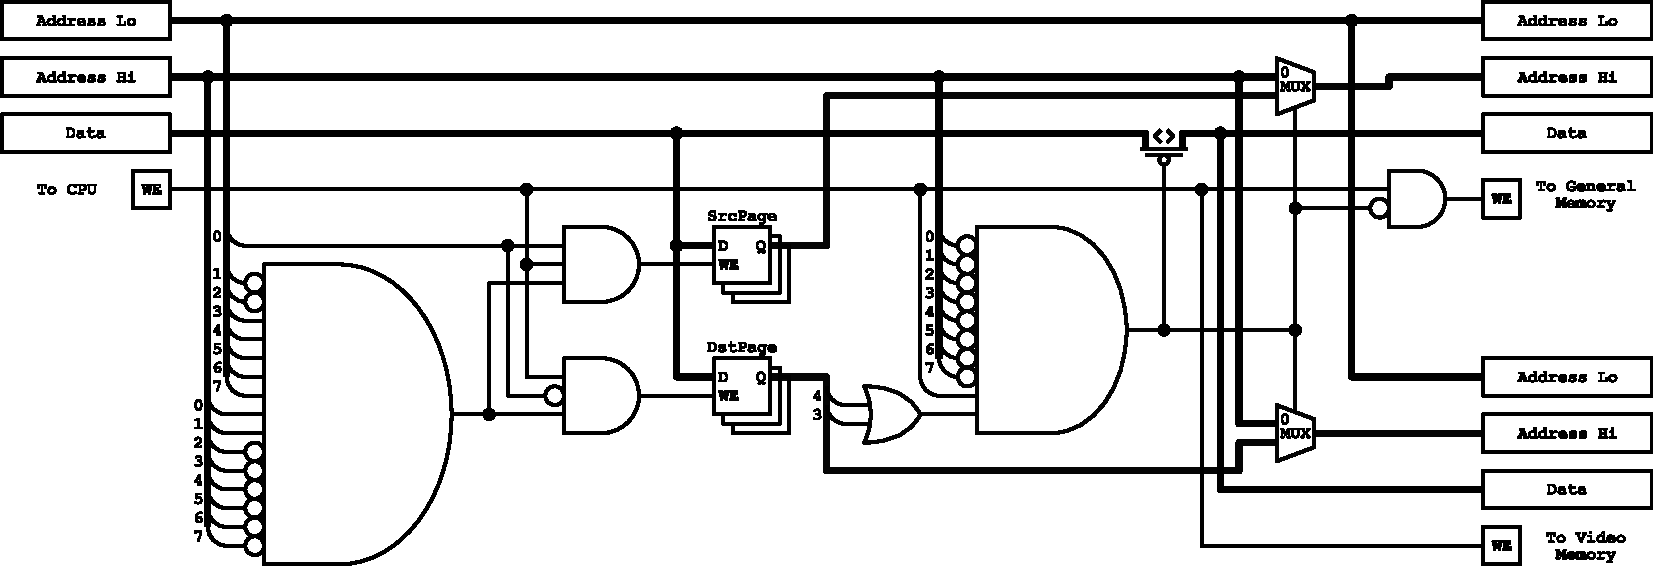
\includegraphics[width=\textwidth]{fvmc}\end{center}

The address bus and write-enable line are forked, with one branch going to the video memory, and the other branch going to all the other memory. The high eight bits of each branch of the address bus are overridden with the contents of the FVMC registers, and the write-enable line is suppressed on the non-video branch. So while the CPU thinks it's writing to zero-page RAM, it's actually triggering a direct memory copy using the data bus, while supplying the low eight bits of the source and destination addresses. Because of a race condition, whether or not the nominally-addressed zero-page memory is changed cannot be garanteed.

The FVMC destination page is set by writing to \texttt{03F8}. Writing a zero to this address disables FVMC. The destination page must be in the range \texttt{08-1F} (video memory) to be effective. The source page is set by writing to \texttt{03F9}, and must not be in the video memory range to be effective.

\section{Interrupts}

Interrupts can be triggered by the video display hardware, as specified by the Video Interrupt Flags, by logic in the cartridge, or by other means not yet determined. In response to an interrupt event, program execution proceeds from address \texttt{2010}.

\chapter{Programming in High-Level Languages}

No programming language interpreter cartridges exist at this time. For now, let's consider this a challenge for the reader.

\cleartoverso
\pagestyle{empty}
\vspace*{\stretch{1}}

\noindent\thetitle\hfill\textcopyright2019--20 \theauthor

\end{document}
